\chapter[Forschungsfrage 1]{Wie können Container-Anwendungen den Prozess des automatisierten \enquote{Deployments} unterstützen?} \label{ff1}
Dieses Kapitel ...

\section{Grundlagen: Definieren der Begrifflichkeiten zur Forschungsfrage eins}
Dieses Teilkapitel soll grundlegende Begrifflichkeiten, die im weiteren Verlauf dieser Arbeit verwendet werden, definieren, um so eine einheitliche Terminologie der Begriffe zu entwickeln. Dadurch wird ein gemeinsames Verständnis erzeugt.

\subsection{Methodik der Anforderungsanalyse}\label{kap:methodikAnfAnalyse}
Die Anforderungsanalyse leitet sich aus dem thematischen Komplex des \enquote{Requirements-Engineering} ab, die verschiedene Bedeutungsvarianten besitzt -- dabei \enquote{[...] steht [es] einmal für alle konkreten Aktivitäten am Beginn einer Systementwicklung, die auf eine Präzisierung der Problemstellung abzielen. Ebenso steht es aber auch für eine ganze Teildisziplin im Grenzbereich zwischen Systems-Engineering, Informatik und Anwendungswissenschaften.}\autocite[][S.\,19]{partsch_requirements-engineering_2010} Diese Analyse soll, laut der herrschenden Meinung der Wissenschaft, am Anfang jeder Systementwicklung stehen, um so bestimmte Vorgehensweise anzuwenden. Dabei entstehen, wenn der später weiter definierte Prozess verfolgt wird, viele systematisch verbundene Dokumente, die Anforderungen enthalten. So ist jede Anforderung wieder ein Cluster von kleineren Anforderungen, die miteinander verbunden sind. Diese werden durch den IEEE-Standard 1220 definiert als \enquote{a statement that identifies a product or process operational, functional, or design characteristic or constraint, which is unambiguous, testable or measurable, and necessary for product or process acceptability (by consumers or internal quality assurance guidelines).}\autocite[][S.\,9]{IEEE1220-2005SystemsEng} Dieser Standard legt mit höchster Priorität den Fokus auf die Formulierung einer Anforderung als elementar wichtig für das Produkt bzw. für das Erreichen der Akzeptanz des Produktes. Ziel der Analyse ist es, funktionale und nicht-funktionale Anforderungen zu identifizieren und diese testbar zu dokumentieren. Funktionale Anforderungen definieren genau, was ein System später erfüllen muss, sie ergeben sich aus der Fragestellung \enquote{Was tut das System?/Was soll es aufgrund der Aufgabenstellung können?}\autocite[][S.\,27]{partsch_requirements-engineering_2010} Nicht-funktionale Anforderungen konkretisieren die Qualitätsansprüche an das System, die Forderung an das zu implementierende System als Ganzes, sowie Randbedingungen, die aus Projekt-/Prozess-/Unternehmensbedingungen resultieren können.\autocite[vgl.][S.\,27-29]{partsch_requirements-engineering_2010}

\begin{figure}[H]
	\centering
	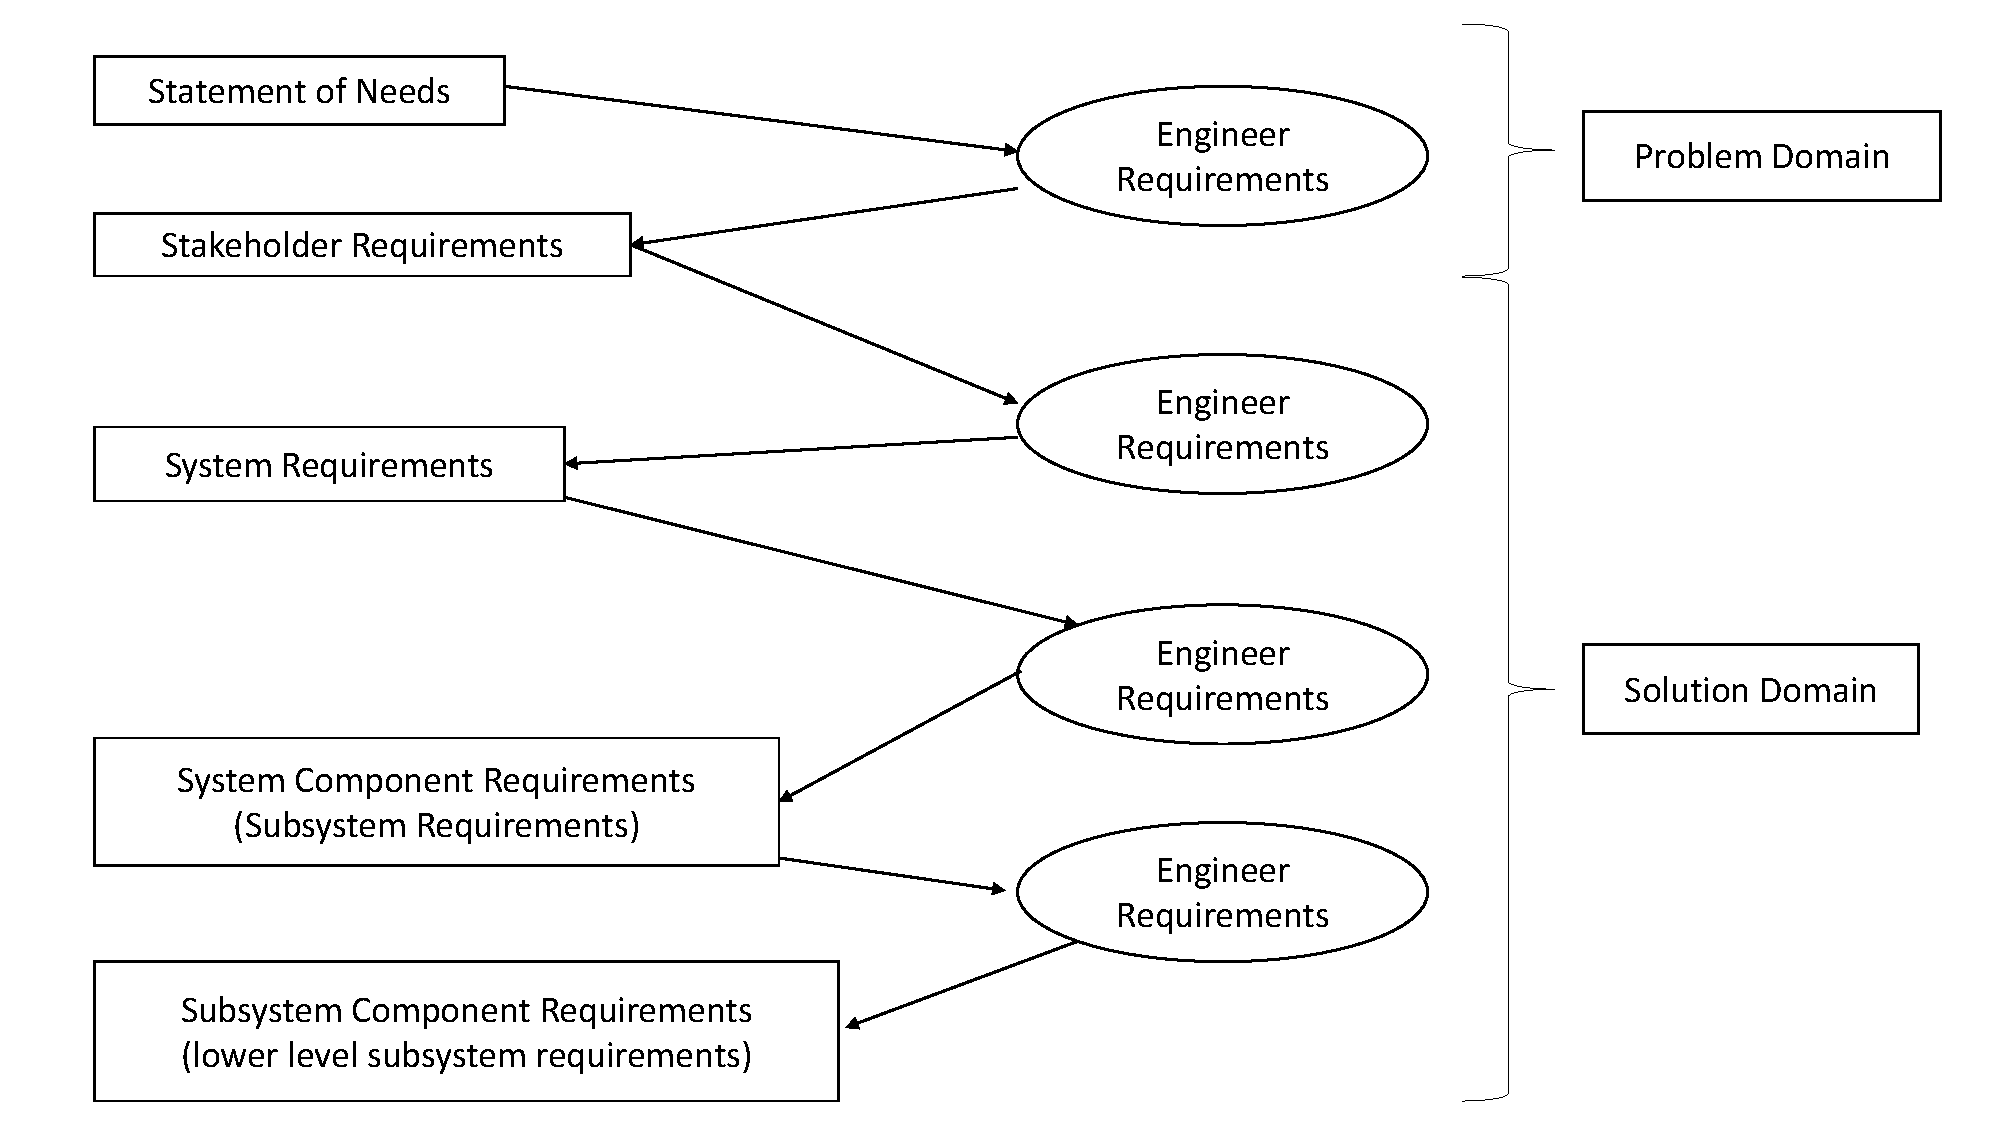
\includegraphics[scale=0.38]{img/levels-of-requirements-engineering.pdf}
	\caption{Entwicklungsprozess der Anforderungen}
	{\footnotesize \cite[Quelle: in Anlehnung an ][S.\,28]{hull_requirements_2011}}
	\label{abb:entwAnforderung}
	%		{\scriptsize \textit{Alle Rechte, einschließlich der Vervielfältigung, Veröffentlichung, Bearbeitung und Übersetzung bleiben der SV Informatik GmbH vorbehalten.}}
\end{figure}

Das \enquote{statement of needs} ist der Startpunkt für die Entwicklung einer Anforderung die am Ende des Prozesses, der in Abbildung \vref{abb:entwAnforderung} dargestellt ist, präzise dokumentiert sein wird. Dieses ist am Anfang immer ein Ausdruck eines Anspruchs oder Wunsches an das zu entwerfende System; dabei bildet das \enquote{statement} und die \enquote{stakeholder requirements} die \enquote{problem domain}. Diese definiert grundständige Methodik, wie auch eine nicht-technische Herangehensweise, die auf die Projektbeteiligten (\enquote{stakeholder}) angepasst ist. Nachfolgend werden die Projektbeteiligen als \enquote{stakeholder} bezeichnen, dabei ist die Rolle beschrieben als \enquote{(Stakeholder) sind Personen oder Organisationen, die ein potenzielles Interesse an einem zukünftigen System haben und somit in der Regel auch Anforderungen an das System stellen.}\autocite[][S.\,8]{partsch_requirements-engineering_2010} Später definiert die \enquote{problem domain} den Zweck des Systems -- dadurch ist bei der Ermittlung der Anforderungen die Frage \enquote{Was ist der Zweck des Systems?} anstelle \enquote{Was soll das System ihrer Meinung nach tun?}. Dies soll die \enquote{stakeholder} extrinsisch motivieren über den Zweck des zu entwerfenden Systems und nicht über einen möglichen Lösungsweg (das Wie) nachzudenken. Durch diesen Ansatz folgen Antworten nach dem Muster \enquote{Ich möchte etwas tun können ...} -- wissenschaftlich bzw. literarisch betrachtet sind diese Form der Anforderungen als \enquote{capability requirement(s)}\autocite[vgl.][S.\,94]{hull_requirements_2011} bekannt. Sie stellen die wichtigsten Erkenntnisse in der \enquote{problem domain} dar. Nun wird im weiteren Verlauf ein Modell konstruiert, das den Projektbeteiligten, den \enquote{stakeholder}, präsentiert wird. Dies unterliegt der Einschränkung, dass es jede/jedem Projektbeteiligte/n versteht. Denn sie validieren das konstruiert Modell in jedem weiteren Schritt, der in Abbildung \vref{abb:entwAnforderung}, ersichtlich ist. Die Anforderungen an das Modell sind quantitativ gering: es muss nicht-technisch sein und es muss geeignet sein die Anforderungen an das System abzubilden. Eine solche Darstellung ist dann geeignet, wenn sie den gewünschten Zweck an das System abbildet, das heißt, dass sie keine technischen Details zeigt, sondern einen Überblick bietet. Ein \enquote{use scenario}\autocite[vgl.][S.\,94]{hull_requirements_2011} wird meist verwendet, da es sich eignet menschliche Aktionen bzw. Ziele darzustellen. Abschließend müssen die \enquote{stakeholder}-Anforderungen folgende Kriterien erfüllen: 

\begin{itemize}
	\item kurz und prägnant formulierte Beschreibung, jedoch einfach zu verstehen und
	\item gleichzeitig sollten sie nicht-technisch, aber realistisch formuliert sein.
\end{itemize}
 
 Die \enquote{solutions domain}, die auf Abbildung \vref{abb:entwAnforderung} zu sehen ist, ist die Nachfolgerin von der \enquote{problem domain}. Der Hauptunterschied zwischen den beiden Bereichen ist, dass die \enquote{solution domain} idealtypisch qualitativ hochwertig beschriebene Anforderungen als \enquote{Input} bekommt. Dazu konträr erhält die \enquote{problem domain} vage formulierte Wunschliste oder einem nicht klar definierten Ziel als initialen \enquote{Input}. Ausgehend von der Aussage von E. Hull, \enquote{in an ideal world, all the requirements would be clearly articulated, individual test able requirements}\autocite[][S.\,115]{hull_requirements_2011}, ist zu deduzieren, dass viele Ebenen zu erforschen gibt, um dieser Aufforderung zu entsprechen. So muss iterativ in jeder Ebene eine neue Analyse des \enquote{Inputs} erfolgen, um einen Ausgangspunkt für das weitere Vorgehen zu initialisieren. Die Komplexität diese Ebenen ist anhängig von dem Grad der Innovation sowie vom Kontext des zu entwickelnden Systems. Jede Entscheidung während des Prozesses kann mögliche Entscheidungspfade in einer anderen Ebene verhindern. Ziel des Prozesses ist es, ein Anforderungsdokument/-katalog zu entwerfen, das laut der gesichteten Literatur in verschiedenen Repräsentationen vorliegen kann. Dennoch sollten primäre Bestandteile, wie die Rahmenbedingungen, die Projektbeteiligten, die Projektaspekte und die funktionale/nicht-funktionale Anforderungen, enthalten sein. Ein Beispiel dieses Katalogs ist im Anhang \vref{appendixAnforderung} zur Ansicht enthalten. Außerdem gibt es im Bereich der Cloud besondere architektonische Anforderungen. Diese sind im Anhang als Abbildung \vref{abb:cloudreq} einzusehen.
 
\subsection{\ac{Cloud-C}}
\ac{Cloud-C}, definiert als: \enquote{Paradigma, einen netzwerkbasierten Zugang auf ein skalierbares und  elastisches Reservoir gemeinsam nutzbarer physikalischer oder virtueller Ressourcen nach dem Selbstbedienungsprinzip und bedarfsgerechter Administration zu ermöglichen}\autocite[][S.\,7]{dindeutsches_institut_fur_normung_informationstechnik_2020-2}, ist ein neuartiger und disruptiver Ansatz in der Informationstechnologie, der seit mehreren Jahren Führungskräfte und IT-Abteilungen beschäftigt. Dieser Ansatz verspricht die Lösung für sämtliche Herausforderungen der Kapazitäts- und Leistungsengpässe moderner IT-Infrastruktur zu sein.\autocite[vgl.][S.\,4]{reinheimer_cloud_2018} Auch diskutiert die Bevölkerung stark und meist auch sehr kontrovers über dieses Thema -- Themen wie Datenschutz und Privatsphäre; Risiko eines Datendiebstahls und die rechtlichen Fragen sind auch nach 20 Jahren Diskussion immer noch allgegenwärtig. Ein Grund dafür ist die hohe Dynamik dieser Technologie, sowie die ständige Weiterentwicklung, die von großen Unternehmen, wie \textsc{Microsoft}, \textsc{Google}, \textsc{Amazon} und \textsc{IBM}, vorangetrieben werden. Momentan haben \textsc{Microsoft} und \textsc{Amazon} die meisten Marktanteile am Umsatz im Bereich des \ac{Cloud-C}.\footnote{siehe dazu Abbildung \vref{abb:marktanteileCC19}} Des Weiteren prognostiziert \cite{gartner_cloud_2019} einen exponentiell wachsenden weltweiten Umsatz bis 2022 auf ungefähr 354,6 Milliarden US-Dollar. Damit würde dieser in den nächsten zwei Jahren um circa 100 Milliarden US-Dollar steigen. Für eine ausführliche Umsatzprognose ist auf die Abbildung \vref{abb:umsatzprognoseCC} zu verweisen. Diese verdeutlicht auch, dass in den folgenden Jahren nach 2022 weiterhin mit einer exponentiellen Umsatzsteigerung zu rechnen ist, wenn das mathematische Modell der exponentiellen Regression weiterhin Bestand hat. 
\par
Historisch betrachtet leitet sich \ac{Cloud-C} an verschiedenen Konzepten anderer \enquote{Comput-ing}-Bereiche und Architekturmustern ab: So spielte zur Entwicklung des heutigen Verständnis \enquote{Utility Computing}, \enquote{Service Orientation} und \enquote{Grid Computing} eine große Rolle.\autocite[vgl.][S.\,3-5]{hill_guide_2013} John McCarthy hat in den 1960er-Jahren das erste Konzept im Bereich des \enquote{Utility Computing} entwickelt.\autocite[vgl.][]{mccarthy_reminiscences_1983} Später wurde es durch Douglas Parkhill verfeinert und durch die folgenden Schlüsselkomponenten beschrieben: \enquote{Parkhill examined the nature of utilities such as water, natural gas and electricity in the way they are provided to create an understanding of the characteristics that computing would require if it was truly a utility. When we consider electricity supply, for example, in the developed world, we tend to take it for granted that the actual electrical power will be available in our dwellings. To access it, we plug our devices into wall sockets and draw the power we need. Every so often we are billed by the electricity supply company, and we pay for what we have used}.\autocite[vgl.][]{parkhill_challenge_1966} Dieses Konzept leitete er auch auf eine technologische Ressource im Bereich des Computers ab.\autocite[vgl.][S.\,4]{hill_guide_2013} Der Gedanke der Serviceorientierung beschreibt eine klare Begrenzung einer Funktion, die zur Erfüllung eines bestimmten Ziels verwendet wird. Services werden meist durch die Konzepte der Objektorientierung und der Abstraktion in einer Organisation definiert. Aus dem Grundgedanken und den genannten Konzepten entwickelt sich die \ac{SOA}, die diese Prinzipien in ein technologiebasiertes Modell abbildet. Die Leitgedanken der \ac{SOA} spielen auch im \ac{Cloud-C} eine wichtige Rolle, denn, wie später noch näher definiert, ist der Servicegedanke ein elementarer Bestandteil der Cloud, der deutlich das Geschäftsmodell prägt. \enquote{Grid Computing} ist ein Konzept aus den 1990er-Jahren und fand seine Anwendung im Bereich der elektrischen Netze.\autocite[vgl.][]{weinhardt_cloud_2009} Ziel dieses Konzeptes war es, die Einfachheit und Zuverlässigkeit der Stromnetze zu gewährleisten über einen standardisierten Adapter Zugriff auf dieses zu erhalten ohne sich um die technische Realisierung kümmern zu müssen. Dabei stellten die Pioniere dieses Konzeptes folgende Eigenschaften\autocite[vgl.][]{foster_grid_1999} an das System:

\begin{itemize}
	\item Dezentrale Ressourcenkontrolle, d.\,h. ein Grid besteht aus geografisch verteilten Ressourcen, die administrativ unabhängig von Organisationen betreut werden.	
	\item Standardisierte, offene Protokolle und Schnittstellen, d.\,h. die Grid-Middleware
	ist nicht anwendungsspezifisch und kann zu verschiedenen Zwecken eingesetzt
	werden.
	\item Nichttriviale Eigenschaften des Dienstes, z. B. in Bezug auf Antwortzeitverhalten, Verfügbarkeit oder Durchsatz.
\end{itemize}
Diese Prinzipien haben eine Ähnlichkeit zu denen des \ac{Cloud-C}, jedoch sind die wirtschaftlichen Aspekte durch die Gedanken des \enquote{Grid Computing} beschrieben. Des Weiteren werden die Aspekte des \enquote{Grid Computings} im Bereich des dezentralen Managements und der verteilten Ressourcen beim \ac{Cloud-C} nicht weiterverfolgt. Vielmehr bietet die Zentralisierung die ökonomischen Vorteile, die eine zentrale Rolle des Geschäftsmodells darstellen. \par
Da es mehrere Definitionen von \ac{Cloud-C} gibt, beschränkt sich diese Arbeit auf folgende: \enquote{Cloud computing is a model for enabling ubiquitous, convenient, on-demand network access to a shared pool of configurable computing resources (e.g., networks, servers, storage, applications, and services) that can be rapidly provisioned and released with minimal management effort or service provider interaction. This cloud model is composed of five essential characteristics, three service models, and four deployment models.}\autocite[][S.\,2]{mell_nist_2011} Das \ac{NIST} beschreibt in der Publikation \cite{mell_nist_2011} folgende essenzielle Charakteristika\footnote{Jedoch werden diese Charakteristika in anderen wissenschaftlichen Ausarbeitungen um \enquote{multitenancy}, \enquote{service oriented} und \enquote{utility-based pricing} ergänzt.\autocite[vgl.][S.\,1]{institute_of_electrical_and_electronics_engineers_cloud_2011}}: 

\begin{itemize}
	\item on-demand self-service
	\item broad network access
	\item resource pooling
	\item rapid elasticity
	\item measured service
\end{itemize}
Des Weiteren beschreibt die \ac{NIST} drei Servicemodelle, wie sich Unternehmen die Cloud zunutze machen können: \ac{SaaS}, \ac{PaaS} und \ac{IaaS}. Dabei wird \ac{SaaS} definiert als: \enquote{The capability  provided to the consumer is to use the provider’s applications running on a cloud infrastructure. [...] The consumer does not manage or control the underlying cloud infrastructure including network, servers, operating systems, storage, or even individual application capabilities, with the possible exception of limited user-specific application configuration settings.}\autocite[][S.\,2]{mell_nist_2011} Cloud-Infrastruktur ist eine Sammlung von Hard-/Software des Cloud-Anbieters, die die fünf essentiellen Charakteristika des \ac{Cloud-C} unterstützt bzw. erfüllt. Beispiele hierfür sind \textsc{Google Docs} und \textsc{Office 365}. \ac{PaaS} wird beschrieben durch: \enquote{The capability provided to the consumer is to deploy onto the cloud infrastructure consumer-created or acquired applications created using programming languages, libraries, services, and tools supported by the provider. The consumer does
not manage or control the underlying cloud infrastructure including network, servers, operating systems, or storage, but has control over the deployed applications and possibly configuration settings for the application-hosting environment.}\autocite[][S.\,2]{mell_nist_2011} Bei der später in der Konzeptionierung verwendeten Software, \textsc{OpenShift}, handelt es sich um eine \ac{PaaS}-Lösung. Weitere Beispiele sind 
\textsc{Google App Engine}, \textsc{Windows Azure} und \textsc{Heroku}.\autocite[vgl.][S.\,8]{kumar_reliability_2018} \ac{IaaS} wird durch folgende Definition abgebildet: \enquote{The capability provided to the consumer is to provision processing, storage, networks, and other fundamental computing resources where the consumer is able to deploy and run arbitrary software, which can include operating systems and applications. The consumer does not manage or control the underlying cloud infrastructure but has control over operating systems, storage, and deployed applications; and possibly limited control of select networking components (e.g. host firewalls).}\autocite[][S.\,3]{mell_nist_2011} Hierzu zählen die Produkte \textsc{Amazon EC2}, \textsc{OpenStack} und \textsc{VMware}. Nun sind die Bereitstellungsmodelle der Cloud noch von Bedeutung -- die \ac{NIST} sowie weitere, schon für diesen Abschnitt verwendete, Literatur definiert vier Modelle: \enquote{private, community, public and hybrid cloud} Die \enquote{private cloud} ist in exklusiver Nutzung eines Unternehmens, dass mehrere interne Konsumenten bedient. Es kann entscheiden, ob alle Management-/Betriebsoperationen intern oder extern von einem Anbieter durchgeführt werden. Die Cloud kann intern oder extern gehostet sein. Die \enquote{community cloud} ist eine \enquote{private cloud}, jedoch unterscheiden sich die beiden durch die Benutzergruppen. Bei der \enquote{community}-Variante ist es nicht auf die Organisation sondern auf Gruppen mit gleichen Angelegenheiten beschränkt. Die \enquote{public cloud} ist offen für die Öffentlichkeit natürlich beschränkt durch die Regel des Cloud-Anbieter. Die hybride Variante wird folgendermaßen beschrieben: \enquote{The cloud infrastructure is a composition of two or more distinct cloud infrastructures (private, community, or public) that remain unique entities, but are bound together by standardized or proprietary technology that enables data and application portability (e.g., cloud bursting for load balancing between clouds).}\autocite[][S.\,3]{mell_nist_2011}


\subsection{Container(-isierung) und Orchestrierung}
\enquote{Historically, virtualization technologies have developed out of the need for scheduling processes as manageable container units. The processes and resources in question are the file system, memory, network, and system information.}\autocite[][S.\,25]{pahl_containerization_2015} Aus dieser Notwendigkeit heraus entstanden verschiedene Lösungsansätze: die Virtualisierung in einer virtuellen Maschine (\ac{VM}) und etwas später die Container-Lösungen. Virtuelle Maschinen konnten einige Herausforderungen, wie \enquote{scheduling, packaging and resource access}, durch ihre technologischen Ansätze lösen. Dabei wurde der architektonische Ansatz des sogenannten \enquote{Gast Systems} entwickelt, d.\,h. die virtuelle Maschine ist ein vollwertiges \ac{OS} mit kompletten Dateisystem und eigenem Prozess auf dem \enquote{Host System}\footnote{bietet Services für die Gastsysteme an}. Im Vergleich dazu können Container die gleichen Anforderung abbilden, jedoch unterscheidet sich die Architektur dieser (vgl. Abbildung \vref{abb:virutalizationArch}). Ein Container enthält alle notwendigen, für die App relevanten, Bibliotheken beziehungsweise Abhängigkeiten und kann so, ohne ein komplettes \ac{OS}, lauffähige Applikationen beinhalten. Diese Abstraktion ist im Cloud-Umfeld (bspw. in einer \ac{PaaS}-Ausprägung) nützlich, da die Container leichtgewichtiger sind und weniger Speicherauslastung (persistenter Speicher) dadurch benötigen. Auch später für die Orchestrierung der Container in einem Cluster-Umfeld ist dies von Nutzen. 

\begin{figure}[H]
	\centering
	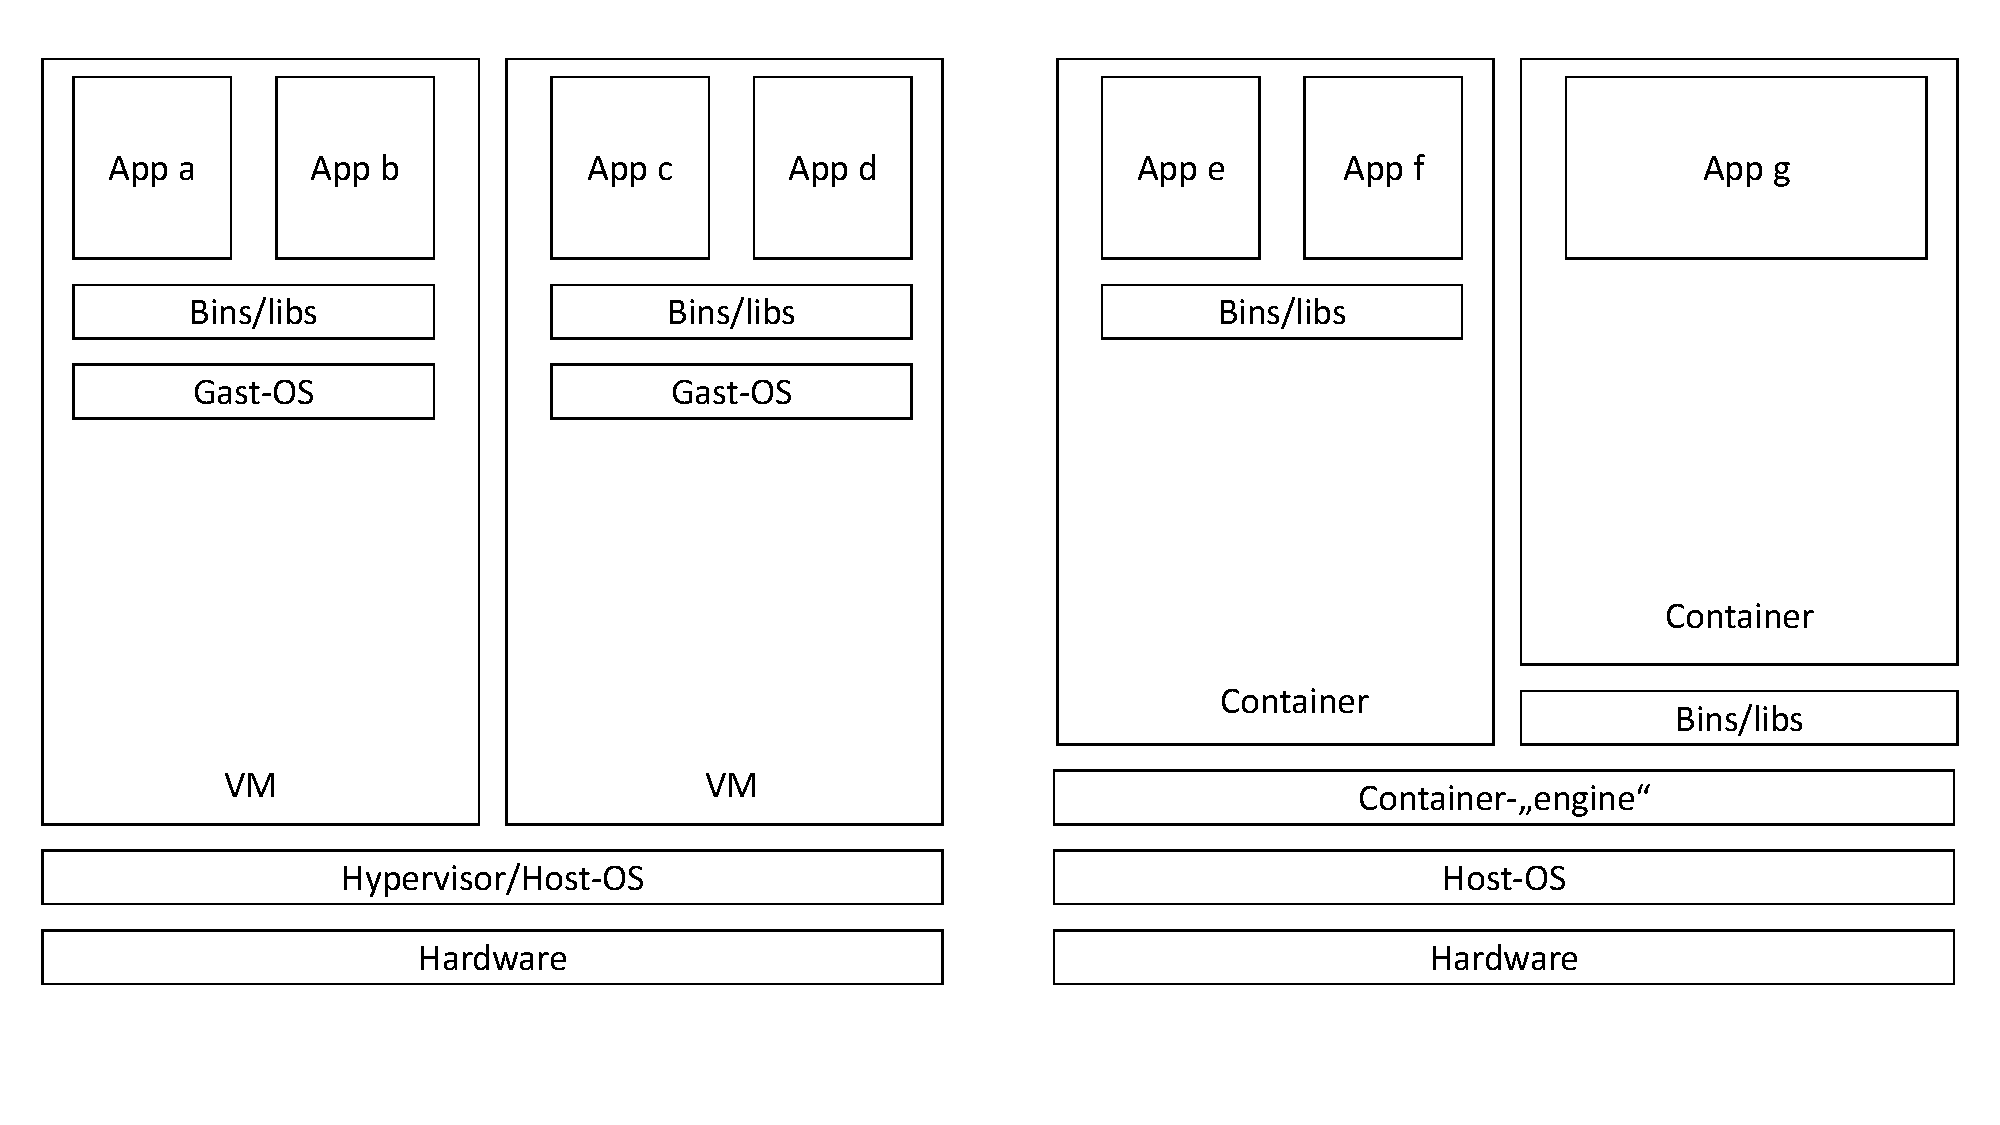
\includegraphics[scale=0.44]{img/virtualization architecture.pdf}
	\caption{Architektur der Virtualisierungsmodelle: VM vs. Container}
	{\footnotesize Quelle: in Anlehnung an \cite{pahl_containerization_2015}}
	\label{abb:virutalizationArch}
	%		{\scriptsize \textit{Alle Rechte, einschließlich der Vervielfältigung, Veröffentlichung, Bearbeitung und Übersetzung bleiben der SV Informatik GmbH vorbehalten.}}
\end{figure}

Die gesichtete Literatur (\cite{pahl_containerization_2015}, \cite{bernstein_containers_2014}, \cite{kharb_automated_2016}; \cite{combe_docker_2016} und weitere siehe Literaturverzeichnis) definieren Container immer anhand ihrer charakteristischen Merkmale und im Vergleich zur \ac{VM}. \cite{google_ireland_limited_container_2020} folgt auch diesem Muster, dennoch eher auf Makroebene: \enquote{Container bieten einen logischen Mechanismus der Paketerstellung, der darauf beruht, dass Anwendungen von ihrer Ausführungsumgebung abstrahiert werden. Mit dieser Entkopplung können containerbasierte Anwendungen einfach und konsistent bereitgestellt werden, unabhängig davon, ob es sich bei der Zielumgebung um ein privates Rechenzentrum, die öffentliche Cloud oder auch um den persönlichen Laptop eines Entwicklers handelt.}\autocite[][]{google_ireland_limited_container_2020} Ziel der Containerisierung ist es, Entwicklerinnen die Möglichkeit zu bieten, sich nur auf die Anwendungslogik und -abhängigkeiten zu konzentrieren. Gleichzeitig können andere IT-Teams, wie \ac{IE2}, sich um die Bereitstellung und Verwaltung dieser Container kümmern. Diese Teams können den Container als geschlossene Verpackung sehen, bei der sie keine Kenntnis über das Innenleben (die Anwendungsdetails) für ihre Arbeit benötigen.\autocite[vgl.][]{google_ireland_limited_container_2020} Dies ist ein Bestandteil der Grundlagen für schnellere und qualitativ hochwertigere Deployments.\autocite[vgl.][S.\,1]{kharb_automated_2016} \par
Initial entwickelte \cite{canonical_ltd_linux_2020} die \ac{LXC}; \textsc{Docker Inc.} ist ein \enquote{open source}-Projekt, dass sich die \ac{LXC}-Technologie zunutze macht und eine Container-\enquote{engine} gebaut hat, um diese Technologie benutzerfreundlicher zu gestalten: \enquote{Basically, \textsc{Docker} extends LXC with a kernel- and application-level API that together run processes in isolation: CPU, memory, I/O, network, and so on. \textsc{Docker} also uses namespaces to completely isolate an application’s view of the underlying operating environment, including process trees, network, user IDs, and file systems.}\autocite[][S.\,82]{bernstein_containers_2014} \textsc{Docker}-Container nutzen eine \enquote{Image}-Struktur. So lassen sich durch Kombination verschiedener \enquote{Images} Applikationen abbilden, die durch Programmierlogik ergänzt werden (vgl. Abbildung \vref{abb:containerArch}). In der Industrie ist \textsc{Docker} als de-facto Standard\autocite[vgl.][S.\,30]{pahl_containerization_2015} angesehen\autocite[vgl.][S.\,1]{kharb_automated_2016}. Außerdem bietet es viele Vorteile, wie die Lichtgewichtigkeit, \enquote{open source}, Sicherheit, Kollaboration zwischen verschiedenen IT-Teams, die Applikation kann überall (wo \textsc{Docker} installiert ist) ausgeführt werden und \textsc{Docker} passt sich an die Unternehmensanforderungen ständig neu an.\autocite[vgl.][S.\,1]{kharb_automated_2016} Durch diese Vorteile entstehen unmittelbare Konsequenzen, die Auswirkungen auf das Arbeiten haben, so wird das Einlernen eines neuen Mitarbeitenden beschleunigt, die Kreativität der Entwicklerinnen verstärkt, die Entwicklungsumgebung vereinheitlicht\footnote{Dies wirkt sich direkt auf die Code-/Produktqualität aus}, die Zusammenarbeit zwischen verschiedenen Teams wird vereinfacht und eine schnelle \enquote{\ac{TTM}}\footnote{\enquote{TTM is the strategy of focusing on reducing the time to introduce new products to market.} (\cite{pawar_time_1994})} wird erreicht.\autocite[vgl.][S.\,2]{kharb_automated_2016} 
\par 
Um die Stärken und Vorteile der \textsc{Docker}-Container, brauchen diese eine Netzwerkanbindung. Nur mit dieser können Container in der Produktion eingesetzt und eine Orchestrierung\footnote{Der Begriff ist aus der Musik abgeleitet: flexibles Kombinieren mehrerer Services oder Dienste zu einer sinnvollen Konzeption (Komposition), die einen Geschäftsprozess beschreibt. Quelle: Duden.de} möglich gemacht werden. Für die Orchestrierung von Container-Anwendungen wird eine weitere Technologie benötigt, die von \cite{google_llc_production-grade_2020} entwickelt und als \enquote{open source} veröffentlicht wurde: \ac{K8s}\footnote{\enquote{is an open-source system for automating deployment, scaling, and management of containerized applications.} (\cite{google_llc_production-grade_2020})}. Die Semantik des Wortes \textsc{Kubernetes} bedeutet auf Griechisch \enquote{Loste/Steuermann}. Diese Metapher beschreibt die Hauptaufgaben von \ac{K8s} zu treffend; es \enquote{verdeckt die Hardwareinfrastruktur und stellt ihr gesamtes Rechenzentrum als eine einzige, enorme Rechenressource dar. Dadurch können Sie ihre Softwarekomponenten	bereitstellen und ausführen, ohne sich darum zu kümmern, welche Server konkret unterhalb dieser Schicht laufen. Bei der Bereitstellung von Anwendungen mit mehreren Komponenten wählt \textsc{Kubernetes} für jede dieser Komponenten einen Server aus, stellt sie bereit und ermöglicht es ihr, die anderen Komponenten zu finden und mit ihnen zu kommunizieren.}\autocite[][S.\,4]{luksa_kubernetes_2018} Der Nutzen von \ac{K8s} wird bei einer großen Cloudanbieterin, wie \ac{AWS} u. a., maximiert, da es den Entwicklerinnen ermöglicht die Ausführung und Bereitstellung von Anwendungen entkoppelt von den Systemadministratorinnen zu betreiben.\autocite[vgl.][S.\,4]{luksa_kubernetes_2018} Eine grundlegende Übersicht einer \textsc{Kubernetes}-Architektur ist im Anhang \vref{abb:k8sArch} zu finden. 
\par
\ac{K8s} führt einige Begrifflichkeiten ein, die nachfolgend einer Definition (siehe Tabelle \vref{tab:definitionenK8s}) benötigen. Diese werden im weiteren Verlauf dieser Arbeit benötigt, jedoch konzentriert auf die Forschungsfrage eins.

\begin{table*}[h!]
	\centering
	\ra{1.3} %more space beetween rules
	
	\begin{tabular}{@{}lp{12.0cm}@{}}\toprule[1.5pt]
		
		\textbf{Begriff} & \textbf{Definition}  \\ \midrule
		% below rules with content
		
		\enquote{Pod} & \enquote{A Pod is a group of one or more tightly coupled Containers sharing a set of Linux namespaces and cgroups.} Innerhalb des \enquote{Pod} wird der Netzwerk-/\enquote{Mount}-Namensraum geteilt, dies ermöglicht die Kommunikationen innerhalb eines \enquote{Pod}. Mehrere dieser kommunizieren über \textit{localhost} \\
		
		\enquote{Services} &  \enquote{A Service is a Kubernetes object that maps one or more incoming ports to targetPorts at a selected set of target of Pods. These represent a microservice or an application running on the cluster.} \\
		
		\enquote{Master nodes} & \enquote{The master nodes are the nodes hosting core elements of the control plane like (not an exhaustive list) the kubeapi-server, kube-scheduler, kube-controller-manager, and in many	instances the etcd database.} Diese übernimmt die Management-Aufgaben im Cluster. \\
		
		\enquote{Worker nodes} & \enquote{The worker nodes (formerly known as minions) host elements like the kubelet, kube-proxy, and the container runtime.} Darin sind die \enquote{Pods} enthalten, welche die Container-Anwendungen beinhalten. \\
		
		\bottomrule[1.5pt]
	\end{tabular}
	
	\caption{Definition der \enquote{\ac{K8s}}-Begrifflichkeiten}
	{\footnotesize{Quelle: \cite[][S.\,10-14]{caban_architecting_2019}}}
	\label{tab:definitionenK8s}
	
\end{table*}
Eine detailreiche Übersicht der Architektur der oben beschrieben Konzepte ist im Anhang \vref{abb:k8sArchInteraktion} zusehen. Diese beschreibt das Zusammenwirkung der einzelnen Komponenten.
% werden zu viele Grundlagen --> wird eine Definition des Deployments benötigt ->
% inline definieren.
%\subsection{\enquote{Deployment}} \label{defDeployment}


\section{Anforderungsanalyse des zu implementierenden Prozess}
% Anforderungskatalog \vref{tab:anforderungslisteFF1}
% Formulierungshilfen für Anforderungen \autocite[][]{rupp_formulierungsregel_2020}
Das \enquote{statement of needs} ist, wie in Kapitel \vref{kap:methodikAnfAnalyse} beschrieben, ein Wunsch beziehungsweise Anspruch an das zu entwickelnde System (hier: ein Prozess): Es sollen Container-Anwendungen automatisiert auf die \textsc{OpenShift}-Umgebung verteilt werden. Dies soll von der dafür zuständigen Abteilung im Unternehmen übernommen werden, d.\,h. die Verantwortung dieses Prozesses wird übergeben. Ziel ist es, Aufgaben und Verantwortlichkeiten so zu verteilen, dass sie dem Aufbau- sowie Ablauforganisation entsprechen. Die Entwicklungsabteilungen/-teams möchten weiterhin nicht mehr für die Verteilung der Container-Anwendungen verantwortlich sein. Des Weiteren sprechen rechtliche Aspekte gegen dies, dass die Entwicklung auf Dauer Anwendungen in die \ac{PROD} verteilt. Bei näherer Betrachtung der oben genannten Gründe ist folgendes festzustellen: es sprechen rechtliche Voraussetzung und unternehmens-organisatorische Aspekte dafür, hier ein weiteres Vorgehen anzustreben. Alleinig durch die rechtlichen Aspekte muss eine Veränderung des IST-Zustands angestrengt werden, damit ist das Vorgehen begründet und die Ermittlung der Projektbeteiligten (\enquote{stakeholder}) kann durchgeführt werden.
\par
Die Projektbeteiligten sind im engeren Sinn die Fachbereiche (also Kunden der Anwendung), die Entwicklungsteams und die \enquote{Deployment}-Abteilung. Im weiteren Sinne könnten die Geschäftsführung der \ac{SVI}, der Vorstand der \ac{SV}, die Kunden der \ac{SV}, sowie die Kunden/der Vorstand der \ac{SVS} ein begründetes Interesse an diesen Projekt haben. So hat der Fachbereich Interesse an einem funktionsfähigen System, die Entwicklungsteams an einem häufigen (annäherungsweise kontinuierlichem) \enquote{Deployment} und die \enquote{Deployment}-Abteilung an einem hoch automatisiertem und revisionskonformen Prozess. Dies sind nur einige Aspekte, die bei weitem nicht alle Gründe des Interesses abdecken. Es werden hier nur die \enquote{stakeholder} im engeren Sinn weiter betrachtet, da diese Arbeit sich mit der Modellierung eines automatisierten Prozesses im Bereich der Entwicklung, der wirtschaftlichen Betrachtung und der rechtlichen Sicherung dieses beschäftigt. Der Fokus liegt auf der Modellierung des Prozesses und mit diesem deckt es die engeren Projektbeteiligten ab. 
\par
Nachfolgend wird der automatisierte \enquote{Deployment}-Prozess zur Verteilung von Containern als \textit{Prozess} bezeichnet. Zur besseren Übersichtlichkeit ist im Anhang \vref{tab:anforderungslisteFF1} ein Anforderungskatalog zu finden. 
% TODO: Definieren welche Anforderungen betrachtet werden --> wahrscheinlich nur die funktionalen Anforderungen ...

- Anforderung von IE2: ARA als Deployment tool

\section{Konzeption eines container-basierten, automatisierten \enquote{Deployments}}
Dieses Teilkapitel beschreibt den Aufbau einer \textsc{OpenShift}-Labor-Umgebung, um das Verhalten von \textsc{OpenShift} zu testen. Des Weiteren wird eine Prozessmodellierung des automatisierten \enquote{Deployments} anhand einer Beispielanwendung \textsc{Camunda} erläutert. Dies ist gleichzeitig die Testapplikation, die in der \ac{SVI} benutzt wird, um das automatisierte \enquote{Deployment} von Container-Anwendungen zu untersuchen. Abschließend wird eine generische Konfigurationsdatei entwickelt, um Applikationen ins \textsc{OpenShift}-Cluster zu verteilen.

\subsection{Aufbau und \enquote{Deployment} eines \textsc{OpenShift}-Labors}
Nachfolgend wird der Aufbau einer \textsc{OpenShift}-Labor-Umgebung mit \enquote{single node}-Architektur beschrieben, d.\,h. es ist nur eine \enquote{worker node} im \textsc{OpenShift}-Cluster vorhanden. Dieses wird auf einem \textsc{Ubuntu}-System in der Version 18.04 installiert. Der folgende Quelltext \vref{lst:openShift} beschreibt die Terminal-Eingaben:

\begin{lstlisting}[language=bash, caption={Installation des \textsc{OpenShift}-Clusters}, label=lst:openShift]
curl -fsSL https://download.docker.com/linux/ubuntu/gpg | sudo apt-key add -
sudo add-apt-repository "deb [arch=amd64] https://download.docker.com/linux/ubuntu $(lsb_release -cs) stable"
sudo apt update && sudo apt -y install docker-ce
docker version
sudo usermod -aG docker $USER
wget $LINK
tar xvf openshift-origin-client-tools*.tar.gz
cd openshift-origin-client*/
sudo mv  oc kubectl  /usr/local/bin/
oc version 
cat << EOF | sudo tee /etc/docker/daemon.json 
{
"insecure-registries" : [ "172.30.0.0/16" ]
}
EOF
sudo systemctl restart docker
oc cluster up
\end{lstlisting}

Das Konzept dieses \enquote{Shell}-Skripts \vref{lst:openShift} ist es, zuerst die notwendigen Abhängigkeiten und danach die \textsc{OpenShift}-Anwendungen zu installieren. So wird in den Zeilen eins bis drei die notwendigen Voraussetzungen geschaffen, um die \textsc{Docker}-Umgebung zu installieren. Zuerst wird der \textsc{GPG}\footnote{\enquote{GnuPG is a complete and free implementation of the OpenPGP standard as defined by RFC4880 (also known as PGP). GnuPG allows you to encrypt and sign your data and communications; it features a versatile key management system, along with access modules for all kinds of public key directories.} Quelle: \cite{the_people_of_the_gnupg_project_gnu_2020}}-Schlüssel zum lokalen Schlüsselbund hinzugefügt, danach kann die Anwendung \textsc{Docker} mit dem \ac{APT}-Programm heruntergeladen und installiert werden. Danach wird getestet, ob die Installation von \textsc{Docker} erfolgreich war und der eigene Benutzer wird der Gruppe \enquote{docker} hinzugefügt. Dies wird benötigt um dem eigenen Benutzer die Steuerung der Software \textsc{Docker} zu erlauben. Die Zeilen sechs bis neun installieren \textsc{Kubernetes} und \textsc{OpenShift} (in der \enquote{Community}-Variante). Sehr wichtig sind die Anpassungen, die in den Zeilen elf bis fünfzehn vorgenommen werden: Sie fügen einen Eintrag \lstinline[language=bash]|"insecure-registries" : [ "172.30.0.0/16" ]| in die Datei \lstinline[language=bash]|/etc/docker/daemon.json| ein. Dies erlaubt es \textsc{Docker} auf unsichere Verzeichnisse zuzugreifen; dadurch kann \textsc{OpenShift} lokal Container-\enquote{Images} im Cache speichern, um diese schneller wiederzuverwenden. Schließlich wird ein Cluster in \enquote{default}-Konfiguration zur Kontrolle der Funktionsfähigkeit mit \lstinline[language=bash]|oc cluster up| erstellt. Dies ist unter \lstinline[language=HTML, breaklines=true]|http://127.0.0.1:8443/console| als Web-Konsole erreichbar.
\par
Um das Verhalten des \textsc{OpenShift}-Clusters während eines \enquote{Deployments} zu testen, wird ein Test-Projekt erstellt. Grundsätzlich sind die meisten Kommandos der \ac{CLI} nach dem Muster \lstinline[language=sh]|oc <action> <object type> <obj name or id>|\autocite[vgl.][]{red_hat_inc_cli_2020} aufgebaut. Ein Projekt ist in \textsc{OpenShift} ein privater Bereich, indem Applikationen laufen können und nur die Erstellerin administrativen Zugriff besitzt. Dieser kann nach außen veröffentlicht werden, wenn dies erforderlich ist. Nachdem das Projekt mit \lstinline[language=bash]|oc new-project <projectName> --display-name '<displayName>'|\footnote{\enquote{<Platzhalter>}, die mit Werten vor der Ausführung ersetzt werden müssen} erstellt wurde, wird dies automatisch als \enquote{default}-Projekt ausgewählt, d.\,h. darin werden nun alle folgenden Schritte ausgeführt. Des Weiteren ist die Überlegung zu treffen, ob noch weitere Benutzer für das angelegte Projekt eine Berechtigung erhalten (\lstinline[language=bash]|oc adm policy add-role-to-user <admin/edit/view> <collabUser>|). 
\par
Als Test-Applikation soll eine Webseite auf Basis von \textsc{Django}\footnote{\enquote{Django is a high-level Python Web framework that encourages rapid development and clean, pragmatic design.} Quelle: \cite[][]{django_software_foundation_web_2020}} in Cluster verteilt werden. Es wird ein vorgefertigtes \enquote{Image} für diesen Test genutzt. Der Quellcode \vref{lst:openShiftDeployLab} zeigt die benötigten Kommandos, um eine neue Applikation zu erstellen. Des Weiteren illustriert dieser, wie die Anwendung nach außen freigegeben wird, d.\,h. sie ist außerhalb des Projektes erreichbar. Danach wird in Zeile \vref{lst:line:testConn} der Quellcode-Abbildung \vref{lst:openShiftDeployLab} die Verbindung zur Webseite mittels der Ermittlung des \textsc{HTTP}-Status-Codes überprüft\footnote{Der Quelltext dieser Funktion ist im Anhang \vref{lst:testConnection} einzusehen}.

\begin{lstlisting}[language=bash, caption={Test-\enquote{Deployment} ins \textsc{OpenShift}-Cluster}, label=lst:openShiftDeployLab]
oc new-app openshiftkatacoda/blog-django-py --name blog
oc describe svc/blog # print config 
oc expose svn/blog
oc status | grep 'to pod port' # see all exposed services on this project

# test_connection is listed at @\vref{lst:testConnection}@
test_connection blog-lab.127.0.0.1.nip.io @\label{lst:line:testConn}@
\end{lstlisting}

Nach Abschluss des Tests wird die Applikation mit \lstinline[language=bash]|oc delete all --selector app=blog| wieder gelöscht.

\subsection{Modellierung einer \enquote{Deployment}-Konfigurationsdatei}
Um eine Verteilung der Container-Anwendung auf dem \textsc{OpenShift}-Cluster durchzuführen, benötigt das System eine Konfigurationsdatei, die als \ac{API}-Objekt an \textsc{OpenShift} übergeben wird. Dabei definiert diese den gewünschten Zustand einer bestimmten Komponente der Anwendung als \enquote{pod}\footnote{siehe Tabelle \vref{tab:definitionenK8s}}-Vorlage.\autocite[vgl.][Application\,$\rightarrow$\,Deployments]{red_hat_inc_okd_2019} Diese Datei stellt, als alleinige Quelle (\ac{SPOT}), alle notwendigen Informationen bereit, die die Anwendungen \textsc{OpenShift} benötigt, um eine funktionsfähige Datei in dem ausgewählten Projekt des Clusters bereitzustellen. Dies ist der erste Unterschied zum klassischen \enquote{Deployment} bei dem alle Quelldateien verteilt werden müssen.\autocite[vgl.][]{dearle_software_2007} Dabei ist die Konfigurationsdatei deklarativ\footnote{Programmierparadigma: im Gegensatz dazu gibt es das imperative Vorgehen, dass das \textit{Was} in welcher Reihenfolge zu tun ist beschreibt.} beschreiben, d.\,h. sie beschreibt \textit{was} \textsc{OpenShift} mit der angegeben Komponente machen soll.

Es gibt zwei verschiedene Ausprägungen der Konfigurationsdatei: \enquote{DeploymentConfig} und \enquote{Deployment}. Nachfolgend werden die Ziele, der Nutzen und ein Beispiel der Ausprägung beschrieben. Die \enquote{DeploymentConfig}-Variante ist von \textsc{Red Hat} für \textsc{OpenShift} entwickelt worden, um eine erweiterte Unterstützung für die Softwareentwicklung und den Lebenszyklus des \enquote{Deployments} zu unterstützen. Damit hat \textsc{Red Hat} ein eigenes Konzept entwickelt, wie die Verteilung von Software aussehen kann. Dieses Konzept bietet folgende Eigenschaften, die verschiedene Nutzungsmöglichkeiten ermöglichen:\autocite[vgl.][Application\,$\rightarrow$\,Deployments]{red_hat_inc_okd_2019}
\begin{enumerate}
	\item \enquote{A DeploymentConfig, which is a template for running applications.}
	\item \enquote{Triggers that drive automated deployments in response to events.}
	\item \enquote{User-customizable deployment strategies to transition from the previous version to the new version. A strategy runs inside a Pod commonly referred as the deployment process.}
	\item \enquote{A set of hooks (lifecycle hooks) for executing custom behavior in different points during the lifecycle of a deployment.}
	\item \enquote{Versioning of your application in order to support rollbacks either manually or automatically in case of deployment failure.}
	\item \enquote{Manual replication scaling and autoscaling.} 
\end{enumerate}
Allgemein definiert das \enquote{DeploymentConfig}-Objekt die Anzahl der Replikationen, beschreibt die Auslöser (\enquote{trigger}) für die automatische Erstellung von neuen \enquote{Deployments}; die Strategie, mit der die Übergange zwischen verschiedenen Versionsständen verwaltet sind, und Lebenszyklus-\enquote{Hooks}\footnote{Funktionen, die beim Eintreten eines bestimmten Events automatisch ausgelöst werden}. Wenn eine neue Verteilung von Komponenten angestoßen wird, aktiviert sich ein spezieller \enquote{pod}, um die die Verteilung zu überwachen und zu betreuen. Dieser fährt die alten Replikationen herunter, aktiviert neue und startet die \enquote{hooks}. Wichtig ist, dass er die alten Replikationen behält, um ein schnelles \enquote{rollback}, also eine Wiederherstellung des Zustands vor der aktuellen Verteilung, zu ermöglichen. Der Verteilungs-\enquote{pod} bleibt für unbestimmte Zeit im Cluster, damit die Logdatei nicht gelöscht wird. 

\lstinputlisting[language=yaml, caption={Beispiel einer \enquote{DeploymentConfig}-Datei}, label=lst:demoDeploymentConfig]{resources/listings/deploymentConfigDemo.yaml}

Dieser Quellcode \vref{lst:demoDeploymentConfig}\autocite[vgl.][Application\,$\rightarrow$\,Deployments]{red_hat_inc_okd_2019} zeigt eine Ausprägung der \enquote{DeploymentConfig}. Die Zeilen 10\,ff. beschreibt typische \enquote{trigger}, die bei einem gewissen Ereignis ausgelöst werden. Die Bezeichner beschreiben die Funktionsweise ausreichend. Die Verteilungsstrategie wird durch die Zeilen 20\,f. eingestellt. Hier wird die Strategie \enquote{rolling} verwendet, d.\,.h die einzelnen \enquote{pods} einer/mehrerer \enquote{worker node(s)} werden während dem laufenden Betrieb unbemerkt gegen die neue Version getauscht -- die Endanwenderin bekommt davon nichts mit. Im Gegensatz zu der Variante \enquote{DeploymentConfig} gibt es die \acl{K8s}-Version \enquote{Deployment}, die kompatibel mit \textsc{OpenShift} ist. Sie werden als Nachkomme der \textsc{OpenShift}-Variante (\enquote{DeploymentConfig})\autocite[vgl.][Application\,$\rightarrow$\,Deployments]{red_hat_inc_okd_2019} bezeichnet. Die \enquote{Deployment}-Ausprägung beschreibt, wie die \enquote{DeploymentConfig}, den gewünschten Zustand einer Anwendungskomponente in Form einer \enquote{pod}-Vorlage. Der Quellcode \vref{lst:demoDeployment}\autocite[vgl.][Application\,$\rightarrow$\,Deployments]{red_hat_inc_okd_2019} erzeugt bei der Ausführung im \textsc{OpenShift}-Cluster eine Replikation des \enquote{hello-openshift}-\enquote{pod}.

\lstinputlisting[language=yaml, caption={Beispiel einer \enquote{Deployment}-Datei}, label=lst:demoDeployment]{resources/listings/deploymentDemo.yaml}

Dabei spezifizieren die Zeilen 16-17, welches \textsc{Docker}-Abbild als Container geladen wird. Die Zeile 19 gibt den Port 80 für die Kommunikation innerhalb des \enquote{pod} frei.
\par
Beide Konfigurationsdatei-Ausprägungen sind vollständig nutzbar in der Anwendungen \textsc{OpenShift}, um eine Verteilung von Komponenten zu beschreiben und auszuführen. \textsc{Red Hat} empfiehlt die Variante \enquote{Deployment} zu nutzen unter der Einschränkung, dass keine Funktionen beziehungsweise kein Verhalten benötigt wird, welches nur die \enquote{DeploymentConfig}-Variante bietet.\autocite[vgl.][Application\,$\rightarrow$\,Deployments]{red_hat_inc_okd_2019} Nachfolgend soll betrachtet werden, welche der möglichen Varianten für die \ac{SVI}, begründet durch die Anforderungen der \enquote{stakeholder}, sinnvoll erscheint. Zuvor werden die beiden Möglichkeiten verglichen und die Unterschiede hervorgehoben: Die Varianten unterschieden sich in einem Punkt sehr stark -- dem Design. Genauer formuliert unterscheiden sie sich in der Eigenschaftsauswahl des CAP-Theorem\footnote{\enquote{The CAP theorem states that any networked shared-data system can have at most two of three desirable properties: consistency (C) equivalent to having a single up-to-date copy of the data; high availability (A) of that data (for updates); and tolerance to network partitions (P).}\autocite[][S.\,1]{brewer_cap_2012} CA macht keinen Sinn, da nicht jeder Client dieselben Daten sehen kann und gleichzeitig immer erreichbar ist.}, so bevorzugt die \enquote{DeploymentConfig}- \enquote{consistency} während die \enquote{Deployment}-Variante \enquote{availability} bevorzugt. Übersetzt bedeutet das, wenn der Verteiler-\enquote{pod} während des \enquote{rollouts} der \enquote{DeploymentConfig} einen Fehler aufweist, wartet der komplette Prozess bis die \enquote{node} mit dem \enquote{pod} wieder aktiv wird oder manuell gelöscht wird. Während dieser Phase stockt der Prozess und es wird kein Fortschritt erreicht. Im Gegensatz dazu wird die Verteilung der \enquote{Deployment}-Variante über einen sogenannten \enquote{controller}-Manager durchgeführt, der als Hochverfügbarkeitslösung implementiert ist, d.\,h. die Verfügbarkeit (\enquote{availability}) steht an erster Stelle. Diese Überlegung muss im Rahmen der Prozessmodellierung als erstes in der \ac{SVI} vollzogen werden, um danach die spezifischen Funktionsunterschiede der beiden Konfigurationsdateien weiter zu beleuchten. 
\par
In einer Arbeitstagung zum \ac{PoC} des \textsc{OpenShift}-Systems haben die Entwicklerinnen einen ersten Entwurf für die Konfigurationsdatei vorgestellt. Hier wurde die Version \enquote{Deployment} verwendet -- begründet war dies durch das Argument, dass keine Funktionen der \enquote{DeploymentConfig}-Version benötigt wurden (Dies ist konform zur Aussage von \textsc{Red Hat}\autocite[vgl.][Application\,$\rightarrow$\,Deployments]{red_hat_inc_okd_2019}). Im Anhang \vref{lst:entwurfCamunda} ist die vollständige Version abgedruckt. Wichtig für den \enquote{stakeholder} Entwicklerin ist, die Beschreibung der Umgebungsvariablen, die die Anwendung braucht, um mit zusätzlichen Webservices zu kommunizieren. Der Quellcode \vref{lst:deploymentCamundaEnv} zeigt diese Stelle nochmals, die einer besonderen Analyse bedarf. Es soll ein Algorithmus zur Generierung der Konfigurationsdateien entwickelt werden. Ziel dieses ist es, mögliche Fehler bei der manuellen Erstellung der Datei zu verhindern und ein vollständig automatisierten Prozess zu entwickeln. Die Generierung mittels Programmlösung ist eine Bedingung der Abteilung \ac{IE2}, die die Verantwortung für die Verteilung der Anwendungen tragen.

\lstinputlisting[language=yaml, firstline=17, lastline=42, firstnumber=17, caption={Ausschnitt aus Quellcode \ref{lst:entwurfCamunda}: Deklaration der Umgebungsvaribalen}, label=lst:deploymentCamundaEnv]{resources/listings/camundaEnv.yaml} 

Die Zeichenketten mit dem Muster \enquote{\textit{\$Bezeichner\_}} stellen Platzhalter dar, die genutzt werden, um die eigentlichen Werte nicht in Klartext abzudrucken. Diese fallen unter das Betriebsgeheimnis. Platzhalter mit der gleichen Zeichenkette haben den identischen Inhalt. Es fällt auf, dass die \ac{URL} der Webservices immer mit dem gleichen Host beginnt und ein Teil des Pfades auch gleich ist. Es gibt zwei Möglichkeiten, wie der Algorithmus zur Generierung der Konfigurationsdateien aussehen könnte: Bei der \enquote{Deployment}-Variante müsste dieser die komplette Datei anhand definierter Regeln generieren. Die zweite Möglichkeit ist die Nutzung eines Vorlagen-Objektes (\enquote{template}), das einmal erstellt, unter gewissen Bedingungen, wiederverwendet werden kann. Dies bedeutet, dass für die Beschreibung der Komponenten-Verteilung die \enquote{DeploymentConfig}-Variante genutzt werden muss, da das \enquote{template}-Objekt nur diese Variante unterstützt. Beides sind Eigenentwicklung von \textsc{Red Hat}. Die Ausprägung \enquote{Deployment} ist ein natives \ac{K8s}-Objekt und deswegen nicht mit dem \enquote{template}-Objekt kompatibel. Es besteht die Möglichkeit diese Objekt mit Parametern zu beschreiben, die in einer Datei \lstinline|<Anwendung>.env| gespeichert und mittels der \ac{CLI} eingelesen werden. Diese ersetzt dann die Parameter mit Werten aus der Datei. Die Entscheidung eine \ac{K-V}-Datei, für die Umgebungsvariablen zu nutzen, hat den Vorteil, dass diese extern in einer verteilten Versionsverwaltungsanwendung (beispielsweise \textsc{Git} oder \textsc{Serena Dimensions}) gespeichert werden kann. Nachfolgend ist der Aufbau einer \ac{K-V}-Datei als Quellcode \vref{lst:envCamunda} für die Umgebungsvariablen des Beispiels \vref{lst:entwurfCamunda} angedeutet. Das Trennzeichen zwischen Schlüssel und Wert ist das Gleichheitszeichen (\enquote{=}). Dieser Aufbau ist verpflichtend, wenn die \ac{CLI} von \textsc{OpenShift} genutzt wird.

\lstinputlisting[language=bash, firstline=7, caption={Umgebungsvariablen als \ac{K-V}-Datei}, label={lst:envCamunda}]{resources/listings/CamundaEnv.env.txt}

Eine Anforderung der Abteilung \ac{IE2} ist es, die Konfigurationsdatei über eine Generierung zu erstellen, um mögliche Syntaxfehler ausschließen zu können. Des Weiteren soll so eine Standardisierung der Konfigurationsdatei unternehmensweit erzielt werden. Das Vorgehen dazu soll folgende Stufen enthalten: 


\begin{enumerate}
	\item Eine einheitliche Übergabedatei soll von den Entwicklungsteams in einer Versionsverwaltung abgelegt werden. Die Datei ist nach Vorgaben der Abteilung \ac{IE2} aufgebaut.
	\item Danach soll aus dieser Datei die Konfigurationsdatei erzeugt werden.
	\item Diese wird durch \textsc{OpenShift} validiert, bevor sie ins Cluster geladen wird.
	\item Das Ergebnis ist die vollständige Konfigurationsdatei, die die Komponenten beschreibt, die verteilt werden sollen.
\end{enumerate}

Für die Generierung ist es wichtig ein Grundgerüst der Konfigurationsdatei zu haben. Dieses ist im Anhang \vref{lst:grundConfig} mit beispielhaften Werten zu sehen. Zweck des Grundaufbau ist es, bei der Generierung die fehlenden Informationen möglichst leicht zu integrieren. Dabei hilft es, wenn eine Grundstruktur des Ergebnisses vorhanden ist. Der Aufbau der zulässigen Wortfolgen in einer Zeile der Übergabedatei ist nachfolgend in der Quellcode-Darstellung \vref{lst:bnfDatei} als \ac{BNF}\footnote{\enquote{Using BNF it is possible to specify which sequences of symbols constitute a syntactically valid program in a given language. (The question of semantics--i.e, what such valid strings of symbols mean--must be specified separately.)}\autocite[][]{mccracken_backus-naur_2003}} beschrieben.

\begin{lstlisting}[language=html, caption={\ac{BNF} der Übergabedatei}, label=lst:bnfDatei, mathescape=true]
	$\langle$Zeile$\rangle$ ::= $\langle$Schluessel$\rangle$ $\langle$Zuweisung$\rangle$  $\langle$Wert$\rangle$ $\langle$EOL$\rangle$ | $\langle$Gruppe$\rangle$ $\langle$EOL$\rangle$ | $\lambda$ $\langle$EOL$\rangle$
	$\langle$Schluessel$\rangle$ ::= $\langle$Grossbuchstaben$\rangle$ | $\langle$Grossbuchstaben$\rangle$ $\langle$Schluessel$\rangle$
	$\langle$Zuweisung$\rangle$ ::= "="
	$\langle$Wert$\rangle$ ::= $\langle$Zeichenkette$\rangle$
	$\langle$Gruppe$\rangle$ ::= "$[$" $\langle$Zeichenfolge$\rangle$ "$]$"
	$\langle$Zeichenfolge$\rangle$ ::= $\langle$Grossbuchstaben$\rangle$ | $\langle$Grossbuchstaben$\rangle$ $\langle$Zeichenfolge$\rangle$
	$\langle$Zeichenkette$\rangle$ ::= $\lambda$ | $\langle$Zeichen$\rangle$ | $\langle$Zeichen$\rangle$ $\langle$Zeichenkette$\rangle$
	$\langle$Grossbuchstaben$\rangle$ ::= "A" | "B" | "C" | "D" | "E" | "F" | "G" | "H" | "I" | "J" | "K" | "L" | "M" | "N" | "O" | "P" | "Q" | "R" | "S" | "T" | "U" | "V" | "W" | "X" | "Y" | "Z" | 
	$\langle$Zeichen$\rangle$ ::= "A" | "B" | "C" | "D" | "E" | "F" | "G" | "H" | "I" | "J" | "K" | "L" | "M" | "N" | "O" | "P" | "Q" | "R" | "S" | "T" | "U" | "V" | "W" | "X" | "Y" | "Z" | "_" | "/" | "-" | ":" | "." | "a" | "b" | "c" | "d" | "e" | "f" | "g" | "h" | "i" | "j" | "k" | "l" | "m" | "n" | "o" | "p" | "q" | "r" | "s" | "t" | "u" | "v" | "w" | "x" | "y" | "z"
\end{lstlisting}
Ein Beispiel einer validen Übergabedatei ist im Anhang \vref{lst:bspUbergabe} zur Veranschaulichung des Konzeptes abgebildet. Nachfolgend beschreibt der Algorithmus \vref{algo:configGenerierung} die Logik zur Generierung einer Konfigurationsdatei. Dieser ist absichtlich in Pseudocode verfasst, um den Fokus auf die Logik zu setzen und nicht auf Besonderheiten einer Programmiersprache. Die Idee dieses ist es, die Übergabedatei einzulesen, auszuwerten und auf Basis dieser eine valide Konfigurationsdatei zu erstellen.

\begin{algorithm}
	\caption{Generierung der Konfigurationsdatei aus einer \ac{K-V}-Datei}\label{algo:configGenerierung}
	
	\begin{algorithmic}
	\Procedure{generateDeploymentConfig}{pathToKVFile}
		\State path $\gets$ pathToKVFile
		\State map$[\quad]$$[\quad]$ \Comment{Map with a key and a value, e.g. a array of lines}
		\State lines$[\quad]$ $\gets$ \Call{ReadFileByLines}{path}
		
		\ForAll{lines$[\quad]$ as line}
			\If{line like \Call{regEx}{"$\backslash[\{1\}([A-Z]+)\backslash]\{1\}$"}}
				\State Test
			\EndIf
		\EndFor
		
	\EndProcedure
	\end{algorithmic}

\end{algorithm}

\subsection{Prozessmodellierung anhand der Anwendung \textsc{Camunda}}
% TODO: Prozessmodellierung schreiben

\section{Ergebnis der Forschungsfrage eins}
% business benefits cloud? --> Teilbereich
- OpenShift Projekte könnten Stages in der Übergangsphase abbilden --> SVI wird immer Stages haben.